\documentclass[10pt,a4paper,conference]{IEEEtran}

% Some very useful LaTeX packages include:
% (uncomment the ones you want to load)

% *** CITATION PACKAGES ***
%
\ifCLASSOPTIONcompsoc
  % IEEE Computer Society needs nocompress option
  % requires cite.sty v4.0 or later (November 2003)
  \usepackage[nocompress]{cite}
\else
  % normal IEEE
  \usepackage{cite}
\fi
% cite.sty was written by Donald Arseneau
% V1.6 and later of IEEEtran pre-defines the format of the cite.sty package
% \cite{} output to follow that of IEEE. Loading the cite package will
% result in citation numbers being automatically sorted and properly
% "compressed/ranged". e.g., [1], [9], [2], [7], [5], [6] without using
% cite.sty will become [1], [2], [5]--[7], [9] using cite.sty. cite.sty's
% \cite will automatically add leading space, if needed. Use cite.sty's
% noadjust option (cite.sty V3.8 and later) if you want to turn this off.
% cite.sty is already installed on most LaTeX systems. Be sure and use
% version 4.0 (2003-05-27) and later if using hyperref.sty. cite.sty does
% not currently provide for hyperlinked citations.
% The latest version can be obtained at:
% http://www.ctan.org/tex-archive/macros/latex/contrib/cite/
% The documentation is contained in the cite.sty file itself.
%
% Note that some packages require special options to format as the Computer
% Society requires. In particular, Computer Society  papers do not use
% compressed citation ranges as is done in typical IEEE papers
% (e.g., [1]-[4]). Instead, they list every citation separately in order
% (e.g., [1], [2], [3], [4]). To get the latter we need to load the cite
% package with the nocompress option which is supported by cite.sty v4.0
% and later. Note also the use of a CLASSOPTION conditional provided by
% IEEEtran.cls V1.7 and later.


% *** GRAPHICS RELATED PACKAGES ***
%
  \usepackage[pdftex]{graphicx}
  \graphicspath{{../Figures/}}
  \DeclareGraphicsExtensions{.pdf,.png}
  \usepackage{color}

% *** MATH PACKAGES ***
%
\usepackage[cmex10]{amsmath}
% A popular package from the American Mathematical Society that provides
% many useful and powerful commands for dealing with mathematics. If using
% it, be sure to load this package with the cmex10 option to ensure that
% only type 1 fonts will utilized at all point sizes. Without this option,
% it is possible that some math symbols, particularly those within
% footnotes, will be rendered in bitmap form which will result in a
% document that can not be IEEE Xplore compliant!
%
% Also, note that the amsmath package sets \interdisplaylinepenalty to 10000
% thus preventing page breaks from occurring within multiline equations. Use:
%\interdisplaylinepenalty=2500
% after loading amsmath to restore such page breaks as IEEEtran.cls normally
% does. amsmath.sty is already installed on most LaTeX systems. The latest
% version and documentation can be obtained at:
% http://www.ctan.org/tex-archive/macros/latex/required/amslatex/math/

%\usepackage{amssymb}%............................ AMS Symbol fonts



% *** SPECIALIZED LIST PACKAGES ***
%
%\usepackage{algorithmic}
% algorithmic.sty was written by Peter Williams and Rogerio Brito.
% This package provides an algorithmic environment for describing algorithms.
% You can use the algorithmic environment in-text or within a figure
% environment to provide for a floating algorithm. Do NOT use the algorithm
% floating environment provided by algorithm.sty (by the same authors) or
% algorithm2e.sty (by Christophe Fiorio) as IEEE does not use dedicated
% algorithm float types and packages that provide these will not provide
% correct IEEE style captions. The latest version and documentation of
% algorithmic.sty can be obtained at:
% http://www.ctan.org/tex-archive/macros/latex/contrib/algorithms/
% There is also a support site at:
% http://algorithms.berlios.de/index.html
% Also of interest may be the (relatively newer and more customizable)
% algorithmicx.sty package by Szasz Janos:
% http://www.ctan.org/tex-archive/macros/latex/contrib/algorithmicx/

% *** ALIGNMENT PACKAGES ***
%
\usepackage{array}
% Frank Mittelbach's and David Carlisle's array.sty patches and improves
% the standard LaTeX2e array and tabular environments to provide better
% appearance and additional user controls. As the default LaTeX2e table
% generation code is lacking to the point of almost being broken with
% respect to the quality of the end results, all users are strongly
% advised to use an enhanced (at the very least that provided by array.sty)
% set of table tools. array.sty is already installed on most systems. The
% latest version and documentation can be obtained at:
% http://www.ctan.org/tex-archive/macros/latex/required/tools/


\usepackage{mdwmath}
\usepackage{mdwtab}
% Also highly recommended is Mark Wooding's extremely powerful MDW tools,
% especially mdwmath.sty and mdwtab.sty which are used to format equations
% and tables, respectively. The MDWtools set is already installed on most
% LaTeX systems. The lastest version and documentation is available at:
% http://www.ctan.org/tex-archive/macros/latex/contrib/mdwtools/

% IEEEtran contains the IEEEeqnarray family of commands that can be used to
% generate multiline equations as well as matrices, tables, etc., of high
% quality.

% *** SUBFIGURE PACKAGES ***
\ifCLASSOPTIONcompsoc
  \usepackage[caption=false,font=normalsize,labelfont=sf,textfont=sf]{subfig}
\else
  \usepackage[caption=false,font=footnotesize]{subfig}
\fi

%Setting captions to centered (Not IEEE journal standard)
%\makeatletter
%\long\def\@makecaption#1#2{\ifx\@captype\@IEEEtablestring%
%\footnotesize\begin{center}{\normalfont\footnotesize #1}\\
%{\normalfont\footnotesize\scshape #2}\end{center}%
%\@IEEEtablecaptionsepspace
%\else
%\@IEEEfigurecaptionsepspace
%\setbox\@tempboxa\hbox{\normalfont\footnotesize {#1.}~~ #2}%
%\ifdim \wd\@tempboxa >\hsize%
%\setbox\@tempboxa\hbox{\normalfont\footnotesize {#1.}~~ }%
%\parbox[t]{\hsize}{\normalfont\footnotesize \noindent\unhbox\@tempboxa#2}%
%\else
%\hbox to\hsize{\normalfont\footnotesize\hfil\box\@tempboxa\hfil}\fi\fi}
%\makeatother


% *** FLOAT PACKAGES ***
%
\usepackage{fixltx2e}
% fixltx2e, the successor to the earlier fix2col.sty, was written by
% Frank Mittelbach and David Carlisle. This package corrects a few problems
% in the LaTeX2e kernel, the most notable of which is that in current
% LaTeX2e releases, the ordering of single and double column floats is not
% guaranteed to be preserved. Thus, an unpatched LaTeX2e can allow a
% single column figure to be placed prior to an earlier double column
% figure. The latest version and documentation can be found at:
% http://www.ctan.org/tex-archive/macros/latex/base/

% *** PDF, URL AND HYPERLINK PACKAGES ***
%
\usepackage{url}

\usepackage{sistyle}
    \SIstyle{S-Africa}
    \SIunitspace{{\cdot}}
    \SIunitdot{{\cdot}}

% generate nice bookmarks and hyperrefs when exporting to pdf and dvi (screen version):
%\usepackage[a4paper,plainpages=false,colorlinks,linktocpage,bookmarks=true,bookmarksopen=false]{hyperref}
% use this for printing only (no color, print version):
%\usepackage[a4paper,plainpages=false,colorlinks=false,linktocpage,bookmarks=true,bookmarksopen=false]{hyperref}
% use this for conference papers where boxes will not look nice. (all colors=black, print version):
\usepackage[a4paper,plainpages=false,colorlinks=true, citecolor=black, filecolor=black, linkcolor=black, pdfhighlight=/O, urlcolor=black, linktocpage,bookmarks=true,bookmarksopen=false]{hyperref}

% correct bad hyphenation here
\hyphenation{op-tical net-works semi-conduc-tor}

%Add elegant support for Big-O notation
\providecommand{\OO}[1]{\operatorname{O}\left(#1\right)}

\begin{document}

%
% paper title
\title{Predicting Object Lifetimes in Finite Distributed Storage Systems Under Churn}

\author{\IEEEauthorblockN{John S. Gilmore and Herman A. Engelbrecht\\
\IEEEauthorblockA{MIH Media Lab, Electrical and Electronic Engineering Department\\
University of Stellenbosch, Stellenbosch, South Africa\\
mail: jgilmore@ml.sun.ac.za and hebrecht@sun.ac.za}}}

\maketitle

\begin{abstract}
%\boldmath
Peer-to-peer network storage systems regularly make use of object replication to achieve sufficient levels of reliability under network churn. To maintain reliability, a repair mechanism is employed, which replaces destroyed replicas. For a given system with an expected churn rate, network size and repair rate, it will be beneficial to know the expected object lifetimes. That is to say, the expected time that an object will remain available in the storage network under known network conditions. This paper proposes an embedded continuous time Markov chain to model objects replicated in a network under churn, with repair. Object lifetimes are found to be dependant on peer departure and arrival rates, initial network size and the maximum network size experienced by an object during its lifetime. The theoretical model results are compared to an Omnet++ network simulation and found to compare favourably.
\end{abstract}

\section{Introduction}
\label{introduction}

Research into distributed systems have received significant research attention over the past few years \cite{}. One of the reasons this has occurred is due to the high costs involved in running centralised systems \cite{}. Centralised systems usually require expensive servers to serve the clients. The interest in distributed systems was initiated by the realisation that for some applications, client machines possess sufficient resources to theoretically serve themselves, thereby removing the need for a server and allowing for significant cost savings \cite{}.

One application of the distributed architecture is the distributed storage system. In centralised storage systems, data are stored on a single machine. The machine can either be a remote data server, or the local machine itself. In attempting to remove the need for a data server, distributed storage systems have been developed. Examples of distributed storage systems include ``Oceanstore'', ``BitTorrent'', ``Freenet'' and ``Past''.

Data stored in a distributed storage system is physically stored on all nodes requiring storage. The issue with this storage scheme is that nodes are connected to the network of their own volition and can leave the network at any time. Nodes joining and leaving the network cause network churn that will eventually destroy any objects stored in the network. The fact that all objects are eventually destroyed, i.e. have a finite lifetime, will be shown by our model in Section \ref{model}.

Because all objects will eventually be destroyed in a distributed storage system, the goal is to design the system so all objects are available for a sufficiently long time. In distributed hash table (DHT) systems, for example, an object usually has a specified time-to-live (TTL), because of the difficulties in deleting objects in the system. Objects in this system just have to live as long as their TTL. In other archival storage systems, objects lifetimes are made longer than the expected lifetime of the systems (thousands of years for example).

In order to design such a storage system, it is therefore of great interest to know the expected lifetime of objects in the system under the expected network conditions and to be able to alter parameters in a predictable way to choose object lifetimes. While other papers, which will be reviewed in Section \ref{related_work}, have also looked at the problem of object lifetimes, none have considered the issue of limited size networks.

In this paper it will be shown that object lifetimes are reduced if the network size is limited, compared to the total number of object replicas stored. While large networks do exist, most networks will practically start out as size limited networks and grow over time as the system gains popularity. Size limited networks have also shown themselves in our research, where we've developed an hierarchical distributed storage system, called Pithos \cite{}. On the second tier of storage, nodes are mapped to a two dimensional Euclidean space and grouped by distance. Each group forms a size limited network, which stores objects. It was found that the lifetime of these objects are affected by the maximum group size during the lifetime of an object.

The paper is structured as follows: Section \ref{background} explains how object storage and repair are generally implemented in a distributed storage system,
%
Section \ref{related_work} discusses other work that has focussed on predicting object lifetimes in distributed storage systems,
%
Section \ref{model} introduces the model that we developed to model object lifetimes,
%
Section \ref{results} presents the results obtained from the model,
%
Section \ref{simulation} briefly introduces the Pithos simulation,
%
Section \ref{comparison} compares the model results with simulation results as well as results from other models and
%
Section \ref{conclusion} concludes.

\section{Background}
\label{background}

When there is referred to a distributed storage system in this paper, it is assumed that there exists some higher layer application that generates objects which it sends to the storage system for storage. The storage system attempts to store an object for as long as possible.

In an attempt to maximise the time an object exists within the storage system, two techniques are used. These are replication and repair.

\subsection{Replication schemes}

There exists two types of what can be termed replication in distributed storage: simple replication and erasure coding \cite{}.

In a storage system using simple replication, $r$ replicas of an object are stored for every object received from the higher layer for storage. Where the number of replicas $r$ is a design decision, which will be discussed in Section \ref{}. This has the effect that an object will remain available until the peer with the longest lifetimes on which it was stored leaves the network, when no repair is done. Intuitively then, it can be expected that the higher the value of $r$, the longer an object will live. This will be shown to be the case in Section \ref{results}.



\subsection{Repair schemes}

\section{Related work}
\label{related_work}

Related work is described, mostly about \cite{replication_article}.

\section{The model}
\label{model}

In order to model the effects of a finite network size on the lifetime of an object, the continuous time Markov chain model introduced in Section \ref{related_work} is expanded by adding a second parameter to every state, namely the network size. This effectively adds another dimension to the Markov chain. The resulting Markov chain is shown in Figure \ref{fig_markov_chain}.

\begin{figure}[htbp]
 \centering
 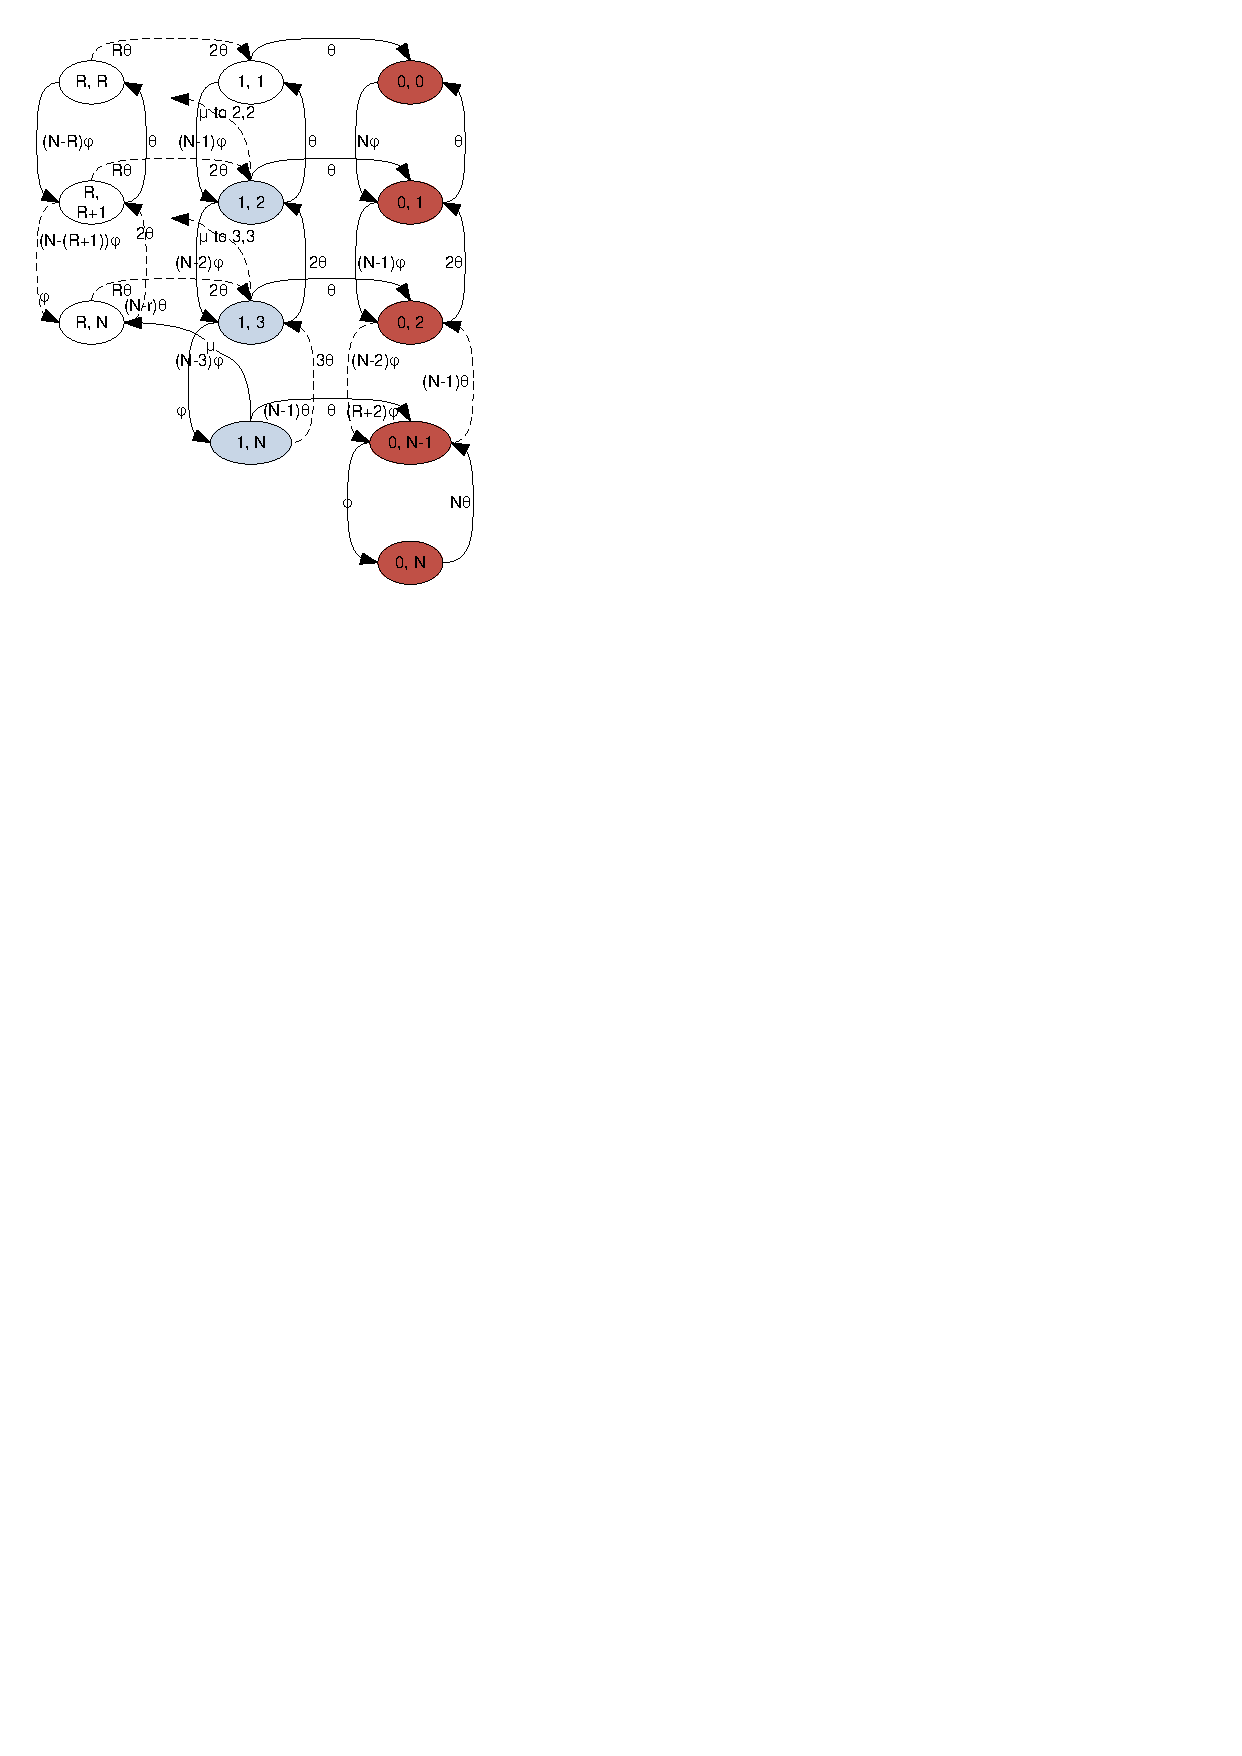
\includegraphics[clip=true, viewport=0.5cm 19.5cm 8.5cm 29.5cm, width=\columnwidth]{Markov_chain_repair_compact}
 \caption{Markov chain modeling object replica number as well as network size}
 \label{fig_markov_chain}
\end{figure}

The dual parameter states can be seen in the Markov chain in Figure \ref{fig_markov_chain}. Every state is a tuple of the form \verb.(replicas,nodes).. Where $r$ is the required number of object replicas and $N$ is the maximum number of nodes in the network. There are four types of transitions possible in our Markov model:
\begin{enumerate}
\item A node that contains a replica departs the network.
\item A node that does not contain a replica departs the network.
\item A node joins the network.
\item An object is repaired.
\end{enumerate}

%In a continous Markov chain we define delta small enough so only one event can occur at any point in time

\begin{figure}[htbp]
 \centering
 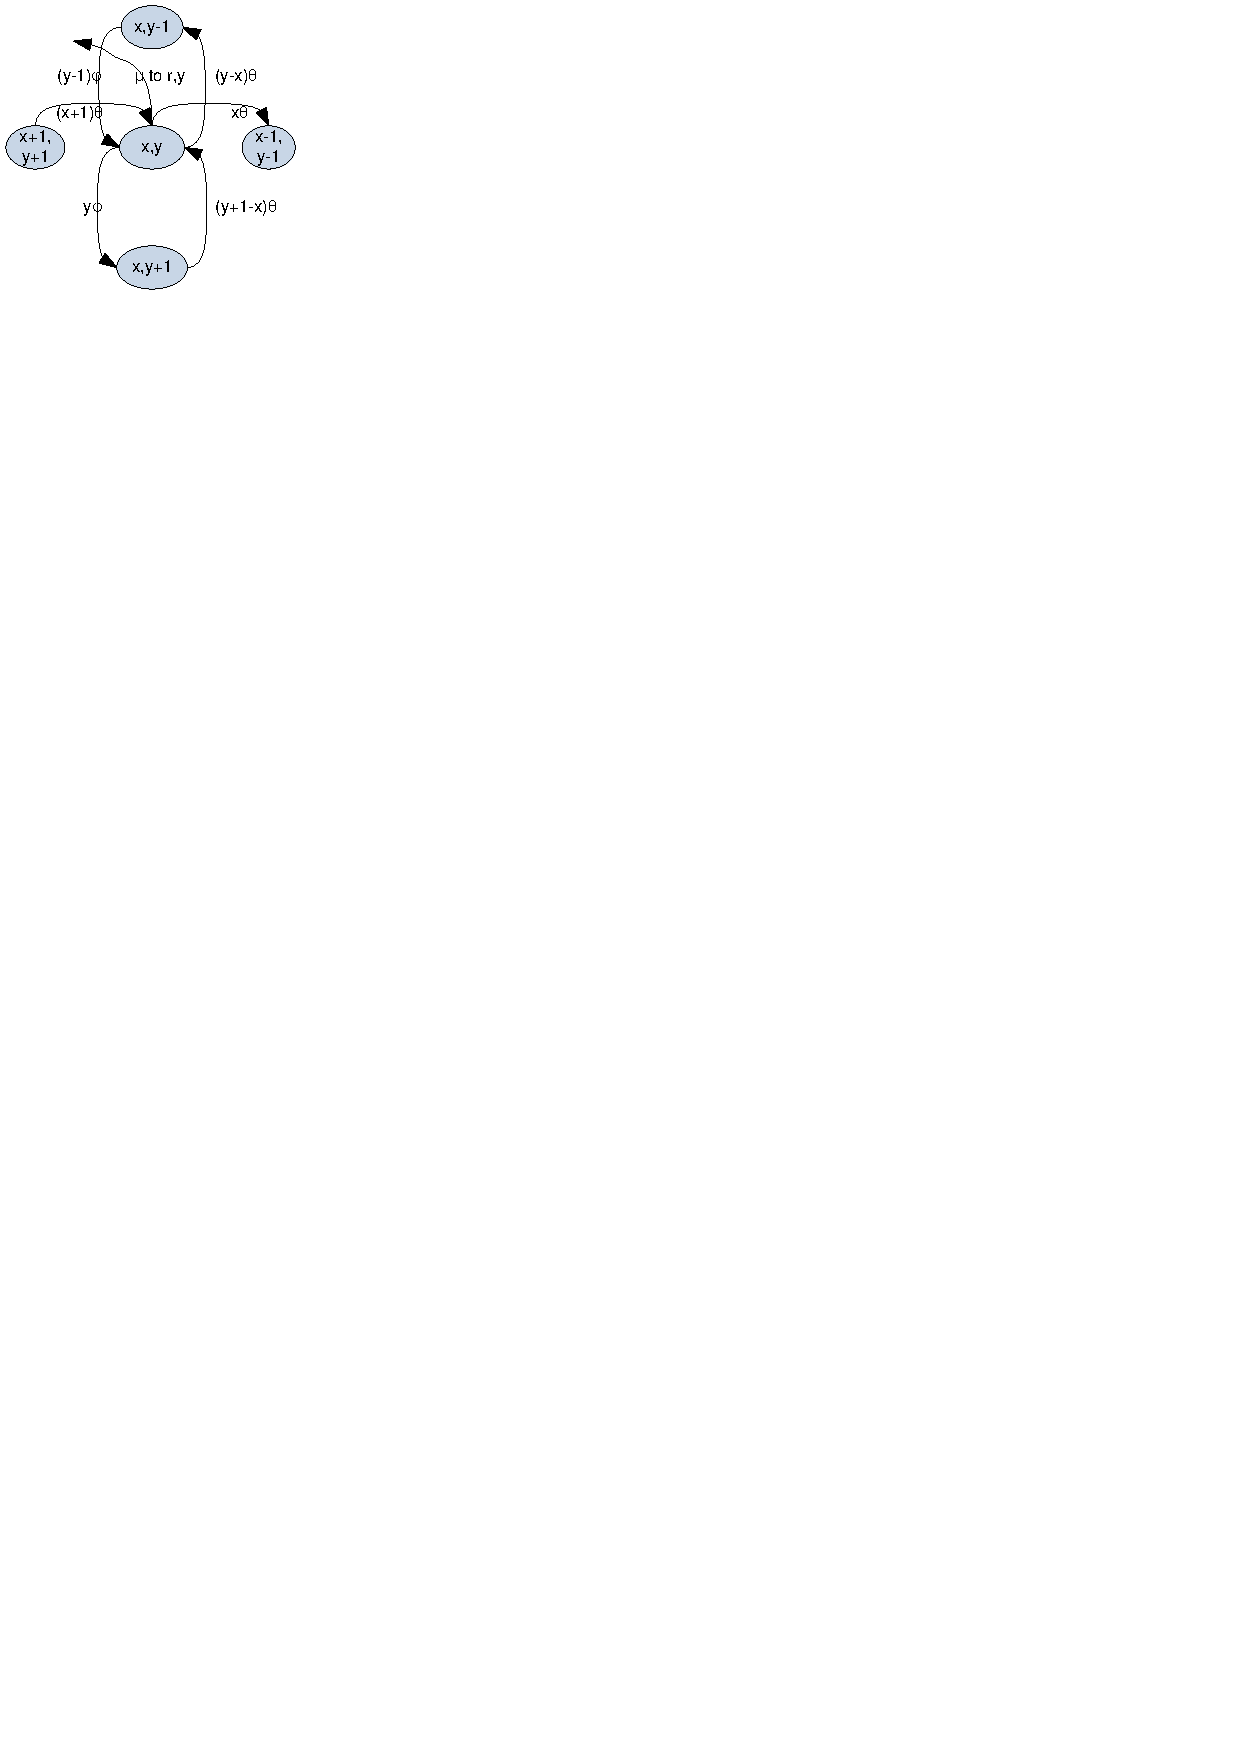
\includegraphics[clip=true, viewport=0.0cm 24.5cm 5.0cm 30cm, width=0.6\columnwidth]{Markov_example}
 \caption{Markov chain modeling object replica number as well as network size}
 \label{fig_markov_example}
\end{figure}

State transitions can be explained by the example in Figure \ref{fig_markov_example}. The figure shows all state transitions relative to the centre state ($x,y$). For the purposes of explanation, only transitions to and from the centre state are shown. Starting at state ($x+1,y+1$), where $x+1$ replicas and $y+1$ nodes are present. If a node that contains a replica departs the network, the system moves to state ($x,y$): one fewer replica and one less node.

If a node that does not contain a replica now departs from the network, the system moves from state ($x,y$) to ($x,y-1$): no fewer replicas and one fewer node. A node can join the network, which will have the model move from ($x,y-1$) to ($x,y$) and another node joining the network will move the system into state ($x,y$+1).

A repair process can also occur. Repair is modeled as a complete repair, which instantly replaces all object replicas if sufficient nodes are available, otherwise it replaces replicas to the number of available nodes. With sufficient nodes available for a full repair, the system moves from state ($x,y$) to ($r,y$) or when the network size is smaller than the required number of replicas the system moves to state ($N,y$).

The transition rates between states are also shown. As with the previous model, the rate at which replicas depart from the network is equal to the product of the number of replicas present in the network at that point in time $r$ and the departure rate of a single peer under steady state $\theta$.

In a continuous time Markov model, moving from one state to the next is characterised by rates, instead of probabilities. This is as opposed to a discrete time Markov model that uses probabilities. Let $\theta$ be the departure rate of nodes under steady state. For $x$ replicas, the node departure rate from the network is then $x\theta$.

The Markov model assumes the presence of a finite sized network, $N$ is chosen sufficiently large.

Taking into account the number of nodes in the network

\begin{equation}
    F(x) = 1 - e^{-\lambda x},\quad\textrm{for}\quad \lambda > 0
\end{equation}

\begin{equation}
    \theta = \lambda
\end{equation}

\begin{equation}
    q(i k,j l) = (N - k)\phi,\quad\textrm{for}\quad i = j,\quad l = k + 1
\end{equation}

\begin{equation}
    q(i k,j l) = i\theta,\quad\textrm{for}\quad j = i - 1,\quad l = k - 1
\end{equation}

\begin{equation}
    q(i k,j l) = (k - i)\theta,\quad\textrm{for}\quad i = j,\quad l = k - 1
\end{equation}

\begin{equation}
    q(i k,j l) = \mu,\quad\textrm{for}\quad i \neq j,\quad l = k,\quad j = \min(r, l)
\end{equation}

\begin{equation}
    q(i k,j l) = 0,\quad\textrm{elsewhere}
\end{equation}

\begin{align}\label{states_num}
       S & = (N - r + 1) + \sum_{x=1}^{r-1} x\notag \\
         & = (N - r + 1) + 0.5 (r - 1) r\notag \\
         & = 0.5 r (2 N - r + 1)
\end{align}

\begin{equation}
    \textbf{P} = \left[\begin{array}{c|c}
                   \textbf{Q} & \textbf{R} \\
                   \hline
                   \textbf{0} & \textbf{I}
                 \end{array}\right]
\end{equation}

\begin{equation}
    \textbf{N} = (\textbf{I} - \textbf{Q})^{-1}
\end{equation}

\begin{equation}
    \textbf{E[L]} = \textbf{Nt}
\end{equation}

\begin{equation}
    \phi = \frac{\tilde{n}\theta}{N - \tilde{n}}
\end{equation}

\section{Model results}
\label{results}

The work is described.

\section{Simulation}
\label{simulation}

The work is described.


\section{Comparison}
\label{comparison}

The work is described.

\section{Conclusion}
\label{conclusion}

We reach some conclusion.

%\newpage
% use section* for acknowledgement
\ifCLASSOPTIONcompsoc
  % The Computer Society usually uses the plural form
  \section*{Acknowledgments}
\else
  % regular IEEE prefers the singular form
  \section*{Acknowledgment}
\fi

The financial assistance of MIH and the National Research Foundation (NRF) towards this research is hereby acknowledged. Opinions expressed and
conclusions arrived at, are those of the author and are not necessarily to be attributed to MIH or the NRF.

%\newpage
%\IEEEtriggeratref{43} %Balance the bibliography
\bibliographystyle{IEEEtran}
\bibliography{../BibTeX/P2P_MMOG}

% that's all folks
\end{document}
